\documentclass[11pt,a4paper]{article}

\usepackage[T1]{fontenc}
\usepackage[utf8]{inputenc}
\usepackage{lmodern}
\usepackage[margin=2.5cm]{geometry}
\usepackage{amsmath,amssymb}
\usepackage{booktabs}
\usepackage{tabularx}
\usepackage{array}
\usepackage{enumitem}
\usepackage{xcolor}
\usepackage{tikz}
\usetikzlibrary{arrows.meta,positioning}
\usepackage[colorlinks=true,linkcolor=blue!60!black,urlcolor=blue!60!black]{hyperref}

\setlist{itemsep=2pt,topsep=4pt}
\newcommand{\code}[1]{\texttt{#1}}
\newcommand{\csat}{c_{\mathrm{sat}}}
\newcommand{\umax}{u_{\max}}

\title{\textbf{DipLabSim Swing-Up to Balance Switching\\Supervisor Design Report}\\[4pt]
\large Lyapunov-Gated Predictive Capture with Hysteretic Fallback\\[2pt]
\normalsize Revision 2: C\# implementation and user interface}
\author{DipLabSim Project Documentation}
\date{November 23, 2026}

\begin{document}
\maketitle

\begin{abstract}
This report presents the design and implementation of the \textbf{Swing-Up Supervisor}
(\code{SwingUpSupervisorController}), a hybrid controller that brings the Double Inverted
Pendulum on a Cart (DIPC) from the hanging position to upright and decides \emph{at run time}
when to hand over from the swing-up law to the existing \textbf{Linear Quadratic Regulator}
(\code{LqrController}). The hand-over is not triggered by fixed angle thresholds. It uses the
LQR's own Riccati matrix $P$ as a Lyapunov function and a short predictive check on the
nonlinear model, with hysteresis for falling back to swing-up. Revision~1 described the design
and a Python prototype. This revision documents the C\# implementation in
\code{DipLabSim.Physics}, its integration into the WPF user interface, the automated tests,
a C\# re-run of the Monte Carlo evaluation, and a comparison with the existing LQR and Cascade
PID controllers. The supervisor is complete and tested for near-upright starts, where it
performs like the LQR; its advantage is that it avoids the rail and can recover after a fall.
The swing-up law itself remains an open item.
\end{abstract}

\tableofcontents
\vspace{6pt}\hrule

\section*{Revision history}
\begin{tabularx}{\linewidth}{@{}l l X@{}}
\toprule
Rev. & Date & Change \\
\midrule
1 & 2026-11-14 & Design and Python prototype evaluation. \\
2 & 2026-11-23 & C\# implementation (branch \code{feat/swingup-supervisor}), user interface
integration, automated tests, C\# Monte Carlo re-run, comparison with the LQR and Cascade PID
controllers, updated open items. \\
\bottomrule
\end{tabularx}

\section{Motivation and Problem Statement}
Both earlier controllers (\code{LqrController}, \code{CascadePidController}) are designed around
the linearized upright model, so they only work near $z = 0$. A full swing-up needs a second,
nonlinear law for large angles, plus a rule that decides when the LQR can take over.

The common rule, $|\theta_1| < \theta_{th}$ and $|\theta_2| < \theta_{th}$, checks the angles
only. It ignores the angular velocities, the cart state and the actuator limit
($\umax = 80$~N). This causes two failure modes:
\begin{itemize}
\item \textbf{Early switch:} the links are near upright but moving fast. The LQR saturates and
the pendulum falls.
\item \textbf{Missed chance:} a state that the LQR could easily catch is rejected because one
angle is slightly above $\theta_{th}$. Swing-up then runs longer than it needs to.
\end{itemize}
The switching rule should therefore answer a dynamic question: \emph{starting from this full
state, will the saturated LQR actually stabilize the system?} It should also adapt
automatically when $Q$, $R$ or the plant parameters change.

\section{Supervisor Architecture (\code{SwingUpSupervisorController})}
\code{SwingUpSupervisorController} implements \code{IController} and wraps two inner laws. Each
control tick it is in exactly one of three modes (enum \code{SupervisorMode},
Figure~\ref{fig:modes}):
\begin{enumerate}
\item \textbf{SwingUp:} a nonlinear law moves the links from the hanging state
($\theta_1 = \theta_2 = \pi$) toward upright. The baseline is energy shaping through collocated
partial feedback linearization (PFL), implemented as \code{EnergyShapingSwingUpController}
(Section~\ref{sec:swingup}).
\item \textbf{Capture:} a short evaluation mode entered when the pre-gate of
Section~\ref{sec:criterion} passes. The swing-up law keeps acting while the capture test runs.
\item \textbf{Balance:} the existing \code{LqrController}, unchanged, regulates the system
around $z = 0$.
\end{enumerate}

\begin{figure}[h]
\centering
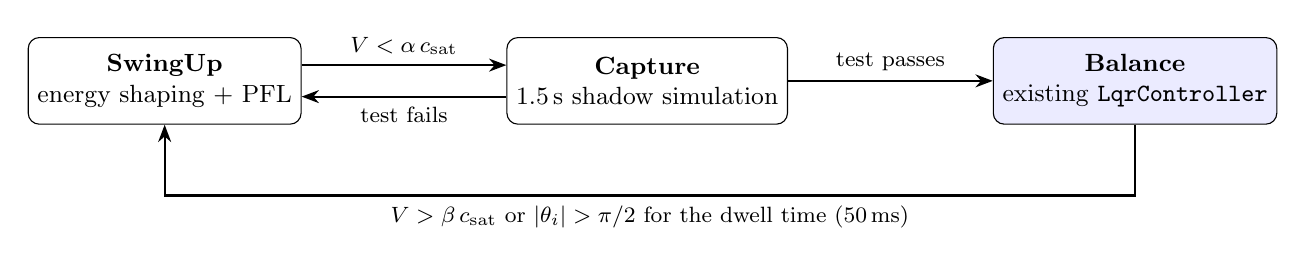
\begin{tikzpicture}[
  node distance=2.6cm,
  mode/.style={draw, rounded corners, align=center, minimum width=3.4cm, minimum height=1.1cm, font=\small},
  arr/.style={-{Stealth[length=2.2mm]}, thick},
  lbl/.style={font=\footnotesize}]
\node[mode] (swing) {\textbf{SwingUp}\\energy shaping + PFL};
\node[mode, right=of swing] (capture) {\textbf{Capture}\\1.5\,s shadow simulation};
\node[mode, right=of capture, fill=blue!8] (balance) {\textbf{Balance}\\existing \code{LqrController}};
\draw[arr] ([yshift=2mm]swing.east) -- node[above, lbl] {$V < \alpha\,\csat$} ([yshift=2mm]capture.west);
\draw[arr] ([yshift=-2mm]capture.west) -- node[below, lbl] {test fails} ([yshift=-2mm]swing.east);
\draw[arr] (capture.east) -- node[above, lbl] {test passes} (balance.west);
\draw[arr] (balance.south) -- ++(0,-0.9) -| node[pos=0.25, below, lbl]
  {$V > \beta\,\csat$ or $|\theta_i| > \pi/2$ for the dwell time (50\,ms)} (swing.south);
\end{tikzpicture}
\caption{Supervisor mode transitions: balance starts only after the capture test passes.}
\label{fig:modes}
\end{figure}

The supervisor does not depend on which swing-up law is used. Its constructor accepts any
\code{IController} as the swing-up stage (the default constructor uses
\code{EnergyShapingSwingUpController}), so the switching logic can be developed and tested
separately from the swing-up design. The supervisor owns and disposes the swing-up controller.
In code, the mode transitions are a single \code{switch} statement in
\code{ComputeControlInput}; there is no table-driven state machine.

\section{Dynamic Switching Criterion}\label{sec:criterion}
The hand-over decision has three layers. Each one runs inside \code{ComputeControlInput}
without heap allocation.

\subsection{Layer 1: Lyapunov Pre-Gate}
\code{DpcLinearizer.SolveLqrGains} iterates the discrete Riccati equation for $P$. It now has an
optional parameter \code{Span<double> pOut}; when it holds at least 36 elements, the converged
row-major $6\times 6$ matrix $P$ is copied into it. Existing callers are unchanged. The
supervisor calls it with the same $Q$, $R$ and plant parameters as its inner LQR, so its $K$
equals the LQR gains exactly. $P$ gives a scalar measure of distance to upright that covers
all six states, with angle errors wrapped to $[-\pi,\pi]$:
\[
V(z) = e^{T} P\, e, \qquad e = z - z_{ref}.
\]
Inside the ellipsoid where the LQR command stays below the actuator limit, the linear design
is valid. The largest such level set has a closed form, so it updates automatically whenever
$Q$, $R$, $\umax$ or the plant change:
\[
\csat = \frac{\umax^{2}}{K P^{-1} K^{T}}.
\]
The pre-gate only checks $V(z) < \alpha\,\csat$, with a wide factor $\alpha$. It is used to
decide when the more expensive Layer~2 test is worth running, not to switch on its own. For the
report-2 plant and the default LQR the C\# implementation gives $\csat = 210.8$ (Python
prototype: $\approx 202$, see Section~\ref{sec:eval}).

\subsection{Layer 2: Predictive Capture Test}
When the pre-gate passes, the supervisor runs a shadow simulation (\code{RunCaptureTest}). It
copies the current state, applies the saturated LQR law to a private
\code{NonlinearEulerLagrangePlant} with \code{Rk4Solver} ($h = 5$~ms, horizon
$T_h = 1.5$~s, i.e.\ 300 steps, cart clamped at $\pm 1.8$~m), and accepts the switch only if
all of the following hold:
\begin{enumerate}
\item $V(z(T_h)) < \rho\, V(z(0)) + 10^{-6}$, meaning the predicted trajectory converges
($\rho = 0.3$). The small absolute floor lets an exactly upright start ($V(0) = 0$) pass.
\item $|\theta_1|, |\theta_2|$ (wrapped) stay below $\pi/2$ throughout the horizon.
\item $|x|$ stays below $1.4$~m, leaving a margin before the rail end.
\end{enumerate}
The simulation stops at the first violation, so a diverging prediction ends early instead of
producing non-finite values. The shadow plant receives the same physical parameters as the
real plant on every \code{Initialize}; link lengths are applied before centre-of-mass
distances, which are clamped to the link length.

The test runs at most once per 10~ms. In the implementation, Capture lasts exactly one control
tick: the tick that enters Capture still applies the swing-up law, and the next tick runs the
test. A pass returns the LQR command on that same tick; a failure returns to SwingUp. Holding
a rejected state at 1~ms ticks therefore runs the test every 11~ms. One full 300-step test
takes about 0.2~ms on a development laptop (Release build), well inside a 1~ms tick.

\subsection{Layer 3: Hysteresis and Fallback}
In Balance mode the supervisor keeps monitoring $V$. If $V > \beta\,\csat$ with
$\beta > \alpha$, or an angle passes $\pi/2$, for at least the dwell time (50~ms), control
returns to SwingUp. The dwell timer accumulates the controller's time step and resets as soon
as the condition clears; at 1~ms ticks the fallback happens on the 50th consecutive violated
tick. Because the entry and exit levels differ and a dwell time is required, the controller
cannot chatter between modes, and a large push during balancing leads to a new swing-up
instead of a fall.

The design did not fix $\beta$. The implementation uses $\beta = 10$ and gives the two factors
disjoint ranges, $\alpha \in [1, 9]$ and $\beta \in [10, 50]$, so $\beta > \alpha$ holds for
every slider setting without rejecting user input at run time.

\section{Swing-Up Law (\code{EnergyShapingSwingUpController})}\label{sec:swingup}
With $d_1,\dots,d_6$ as in the plant, the pendulum energy in the cart frame is
\[
E_p = \tfrac12\left(d_4\dot\theta_1^2 + d_6\dot\theta_2^2\right)
 + d_5\cos(\theta_1-\theta_2)\,\dot\theta_1\dot\theta_2
 + g\left(d_2\cos\theta_1 + d_3\cos\theta_2\right),
\qquad E_{up} = g\,(d_2 + d_3).
\]
Without damping, $\dot E_p = -\ddot x\, w$ with
$w = d_2\cos\theta_1\,\dot\theta_1 + d_3\cos\theta_2\,\dot\theta_2$. The desired cart acceleration
\[
a = \operatorname{sat}_{a_{\max}}\!\Big(k_E\,(E_p - E_{up})\,\tilde w
 - k_x\,(x - x_{ref}) - k_v\,\dot x\Big)
\]
therefore drives $E_p$ toward $E_{up}$ while a weak PD term keeps the cart centred. At hanging
rest $w = 0$ and the pumping term would vanish, so $\tilde w = w$ for $|w| \ge 0.05$ and
$\tilde w = \pm 0.05$ (sign of $w$, positive at zero) otherwise. Collocated PFL then fixes
$\ddot x = a$, solves the $2\times 2$ link block of $M(q)\ddot q = \ldots$ for
$\ddot\theta_1, \ddot\theta_2$, and reads the force $u$ from the cart row, including the viscous
damping terms $b$, $c_1$, $c_2$. The result is clamped to $\pm\umax$.

\begin{table}[h]
\centering
\begin{tabular}{@{}l l l l l@{}}
\toprule
Key & Symbol & Default & Range & Unit \\
\midrule
\code{KEnergy} & $k_E$ & 0.3 & 0--5 & 1/(J\,s) \\
\code{KCartX} & $k_x$ & 2.0 & 0--50 & 1/s$^2$ \\
\code{KCartV} & $k_v$ & 3.0 & 0--50 & 1/s \\
\code{MaxAccel} & $a_{\max}$ & 15 & 0.5--50 & m/s$^2$ \\
\code{MaxForce} & $\umax$ & 80 & 5--100 & N \\
\bottomrule
\end{tabular}
\caption{Swing-up law parameters. The supervisor forwards its own $\umax$ to this law and to
the inner LQR. These parameters are not yet shown in the user interface.}
\label{tab:swingup}
\end{table}

\section{User Interface Integration}\label{sec:ui}
The supervisor is registered in \code{MainViewModel.AvailableControllers}. No XAML change was
needed: the existing data-driven controller panel builds its rows from the controller's
\code{ParameterDescriptor} list.
\begin{itemize}
\item \textbf{Controller selector:} the drop-down now has four entries: LQR, Cascade PID,
\emph{Swing-Up Supervisor (Energy PFL $\rightarrow$ LQR)} and None (Open-Loop).
\item \textbf{Parameter panel:} selecting the supervisor shows the six parameters of
Table~\ref{tab:uiparams} under the group \emph{Swing-Up Supervisor}, each with a slider and a
numeric box. As for the other controllers, edits are made while the simulation is paused.
\item \textbf{Gains summary:} shows the current mode, $V/\csat$, $\csat$ and the LQR gain vector,
for example \code{Mode: Balance | V/c\_sat = 0.12 | c\_sat = 210.8 | K = [...]}. While the
supervisor is selected the summary is refreshed on every rendered frame, so mode changes are
visible during a run.
\item \textbf{Auto-calculate:} re-tunes the inner LQR weights for the current plant (the same
Bryson-scaled rule as \code{LqrController}) and rebuilds $P$ and $\csat$.
\item \textbf{Reset to defaults:} restores the supervisor parameters and the inner LQR weights.
\item \textbf{Initial state presets:} \emph{Upright} and \emph{Perturbed} reach Balance within two
ticks; \emph{Hanging} starts in SwingUp.
\end{itemize}

\begin{table}[h]
\centering
\begin{tabular}{@{}l l l l l l@{}}
\toprule
Key & Symbol & Default & Range & Step & Meaning \\
\midrule
\code{Alpha} & $\alpha$ & 5.0 & 1--9 & 0.1 & pre-gate $V < \alpha\,\csat$ \\
\code{Beta} & $\beta$ & 10.0 & 10--50 & 0.5 & fallback $V > \beta\,\csat$ \\
\code{HorizonTh} & $T_h$ & 1.5~s & 0.25--5~s & 0.05 & capture test horizon \\
\code{Rho} & $\rho$ & 0.3 & 0.01--0.99 & 0.01 & required decay of $V$ over $T_h$ \\
\code{DwellTime} & $t_{dwell}$ & 0.05~s & 0--0.5~s & 0.005 & fallback dwell time \\
\code{MaxForce} & $\umax$ & 80~N & 5--100~N & 1 & actuator limit, used in $\csat$ \\
\bottomrule
\end{tabular}
\caption{Supervisor parameters exposed in the user interface.}
\label{tab:uiparams}
\end{table}

Not yet implemented in the user interface: the planned $V(t)$ trace on the telemetry scope, and
the swing-up law parameters of Table~\ref{tab:swingup}.

\section{Evaluation}\label{sec:eval}
\subsection{Python prototype (Revision 1)}
In the prototype, the predictive test never switched too early and found 85\% of the
catchable states. The fixed angle threshold caused a failed hand-over in 44\% of its switches.

\textbf{Setup.} A Python port of \code{NonlinearEulerLagrangePlant} was used with report-2
parameters, the default LQR ($Q = \mathrm{diag}(12, 60, 120, 8, 6, 12)$, $R = 1$) and
$\umax = 80$~N. We drew 300 random near-upright states in the band a swing-up passes through:
$|x| \le 0.5$~m, $|\theta_1|, |\theta_2| \le 0.4$~rad, $|\dot x| \le 1$~m/s,
$|\dot\theta_1|, |\dot\theta_2| \le 2.5$~rad/s. The ground truth for each state was a 10~s
closed-loop LQR run with RK4 at 2~ms, counted as a success if $V < 0.5$ at the end and the
rail end was never reached. 142 of the 300 states (47\%) were catchable.

\subsection{C\# implementation (Revision 2)}
The same experiment was repeated against the C\# classes with the same band, ground truth and
defaults (300 states, a different random draw). 147 of the 300 states (49\%) were catchable.
Every catchable state was inside the $\alpha = 5$ pre-gate, as in the prototype. This run was a
one-off check; its script is not part of the repository.

\begin{table}[h]
\centering
\begin{tabular}{@{}l rrrr rrrr@{}}
\toprule
 & \multicolumn{4}{c}{Python prototype (142 catchable)} & \multicolumn{4}{c}{C\# (147 catchable)} \\
\cmidrule(lr){2-5}\cmidrule(lr){6-9}
Criterion & Sw. & Failed & Prec. & Rec. & Sw. & Failed & Prec. & Rec. \\
\midrule
Fixed angles, $|\theta_i| < 0.3$~rad & 182 & 80 & 0.56 & 0.72 & 173 & 78 & 0.55 & 0.65 \\
Lyapunov gate only, $V < \csat$ & 70 & 0 & 1.00 & 0.49 & 82 & 0 & 1.00 & 0.56 \\
Pre-gate ($\alpha = 5$) + predictive test & 121 & 0 & 1.00 & 0.85 & 127 & 0 & 1.00 & 0.86 \\
\bottomrule
\end{tabular}
\caption{Switching criteria on 300 Monte Carlo states.}
\label{tab:montecarlo}
\end{table}

The C\# results confirm the prototype: the Lyapunov gate alone is safe but conservative, and the
combined criterion keeps zero failed switches while recovering most catchable states. $\csat$ is
210.8 in C\# against $\approx 202$ in the prototype; the cause of this 4\% difference has not
been investigated.

\subsection{Automated tests}
Table~\ref{tab:tests} lists the four tests planned in Revision~1, now in
\code{DipLabSim.Numerics.Tests/SwingUpSupervisorTests.cs}. The test states were chosen from the
Monte Carlo band and checked against the LQR ground truth. In addition, the supervisor was added
to the existing near-upright stabilization test (both plant models, start
$(x,\theta_1,\theta_2) = (0.25, 0.06, -0.05)$, 8~s), where it meets the same tolerances as the
plain LQR. The user-interface acceptance test now expects four controllers and checks the six
supervisor parameters. All 51 numerical tests (Debug and Release) and all 7 user-interface tests
pass.

\begin{table}[h]
\centering
\begin{tabularx}{\linewidth}{@{}>{\raggedright\arraybackslash}p{3.6cm} X@{}}
\toprule
Test & Check \\
\midrule
No switch from a fast, uncatchable state &
$z = (0, 0.1, 0.15, 1.0, 2.5, -0.5)$: inside the fixed angle threshold and the pre-gate
($V/\csat = 1.78$), but the LQR cannot catch it. Held for 30 ticks, the supervisor never enters
Balance and runs 2--4 capture tests (rate limit). \\
Switch from a slow state outside the angle threshold &
$z = (-0.3, 0.32, 0.36, 0, 0, 0)$: both angles above 0.3~rad and $V/\csat = 1.19$, so the
Lyapunov gate alone would reject it. Balance within 5 ticks, never left during 10~s, final
state within $|x| < 0.02$~m, $|\theta_i| < 0.01$~rad. \\
Fallback after a large tip push &
From upright: a 2~N, 80~ms push keeps Balance. A 40~N, 200~ms upper-tip push returns to SwingUp,
and only after the dwell time has elapsed since the first violation. \\
Zero allocation over 1\,000 ticks &
300 hanging ticks (SwingUp), 400 ticks of repeated rejected capture tests, 300 ticks ending in
Balance; at least 30 capture tests inside the measured window; 0 bytes allocated. \\
\bottomrule
\end{tabularx}
\caption{Supervisor tests.}
\label{tab:tests}
\end{table}

\subsection{Swing-up from hanging}
Revision~1 reported that the energy-shaping baseline brought $E_p$ to $E_{up}$ in about 3~s and
then wandered chaotically without entering the LQR basin within 20~s. With the C\# law and the
default gains of Table~\ref{tab:swingup}, a single deterministic 60~s run from
$\theta_1 = \theta_2 = \pi$ at rest (1~ms steps, RK4) gave:
\begin{itemize}
\item $E_p$ within 5\% of $E_{up}$ after 8.6~s;
\item 51 entries into Capture before the first accepted hand-over at 22.7~s;
\item no fallback afterwards, final state upright (angles modulo $2\pi$), $|x| \le 1.03$~m
throughout.
\end{itemize}
This is one run with one parameter set and no automated test covers it. It shows that the
supervisor hands over correctly when the swing-up law happens to pass through the basin, not
that the swing-up problem is solved.

\section{Comparison with the Other Controllers}\label{sec:compare}
The supervisor was compared with the two existing balancing controllers, \code{LqrController}
and \code{CascadePidController}, under identical conditions: the engine's
\code{SimulationLoop} with RK4 at 1~ms, report-2 plant parameters, default controller
parameters ($\umax = 80$~N), the engine's total force clamp of $\pm 100$~N and its rail at
$\pm 1.8$~m (velocity set to zero at contact). A run counts as a success when $V < 0.5$ at the
end (angles modulo $2\pi$) and the cart never touched the rail end. The open-loop controller
applies no force and falls from every state below, so it is not listed. All runs are single
deterministic simulations made with a one-off script that is not part of the repository.

\begin{table}[h]
\centering
\begin{tabularx}{\linewidth}{@{}X ccc@{}}
\toprule
Scenario & LQR & Cascade PID & Supervisor \\
\midrule
\multicolumn{4}{@{}l}{\emph{Monte Carlo band of Section~\ref{sec:eval}, 300 states, 10~s}} \\
\quad Successes & 147 & 143 & \textbf{189} \\
\quad Runs with rail contact & 153 & 157 & \textbf{0} \\
\midrule
\multicolumn{4}{@{}l}{\emph{Start $(x,\theta_1,\theta_2) = (0.25, 0.06, -0.05)$, at rest, 10~s}} \\
\quad Settling time$^{*}$ [s] & 4.86 & 5.06 & 4.87 \\
\quad Peak $|u|$ [N] & 30.0 & 29.7 & 30.4 \\
\quad Peak $|x|$ [m] & 0.340 & 0.340 & 0.341 \\
\quad Control effort $\int u^2\,dt$ [N$^2$s] & 38.3 & 38.1 & 39.2 \\
\midrule
\multicolumn{4}{@{}l}{\emph{Start $(0, 0.2, 0.2)$, at rest, 10~s}} \\
\quad Settling time$^{*}$ [s] & 5.15 & 5.34 & 5.15 \\
\quad Peak $|u|$ [N] & 13.9 & 13.6 & 13.9 \\
\quad Peak $|x|$ [m] & 0.868 & 0.892 & 0.869 \\
\quad Control effort [N$^2$s] & 47.1 & 45.4 & 47.1 \\
\midrule
\multicolumn{4}{@{}l}{\emph{100~ms tip push at $t = 0.5$~s from upright, 15~s}} \\
\quad Largest push held in balance, upper tip [N] & 2.4 & 2.4 & 2.4 \\
\quad Largest push held in balance, lower tip [N] & 3.8 & 3.8 & 3.8 \\
\quad Upright again at 15~s after a 4--40~N upper-tip push (19 runs) & 0 & 0 & \textbf{9} \\
\quad Upright again at 15~s after a 4--40~N lower-tip push (19 runs) & 0 & 0 & \textbf{7} \\
\quad Rail contact in those 38 runs & 38 & 38 & \textbf{3} \\
\midrule
\multicolumn{4}{@{}l}{\emph{Start hanging, $\theta_1 = \theta_2 = \pi$, at rest, 60~s}} \\
\quad Upright at the end & no & no & \textbf{yes (from 22.7~s)} \\
\quad Rail contact & yes & yes & no \\
\midrule
\multicolumn{4}{@{}l}{\emph{Cost of \code{ComputeControlInput} (Release, development laptop)}} \\
\quad Steady state [ns per call] & 82 & 19 & 78 \\
\quad Capture-test tick [ms] & -- & -- & $\approx 0.2$ \\
\quad Heap allocation per call [bytes] & 0 & 0 & 0 \\
\bottomrule
\end{tabularx}
\par\smallskip
{\footnotesize $^{*}$Last time the state was outside $|x| < 0.02$~m,
$|\theta_1|, |\theta_2| < 0.01$~rad. Push forces were swept in steps of 0.1~N for the
thresholds and 2~N for the 4--40~N range.}
\caption{Supervisor compared with the existing controllers.}
\label{tab:compare}
\end{table}

\textbf{Near upright the supervisor is the LQR.} From states the LQR can catch, the supervisor
reaches Balance after two ticks and from then on applies the unchanged \code{LqrController}
law, so settling time, peak force, cart travel and control effort match the LQR to within the
effect of those first two swing-up ticks. The Cascade PID gains are factored from an LQR design
with slightly different weights, which is why it behaves almost the same and settles about
0.2~s later. The supervisor does not enlarge the set of disturbances that can be rejected
without falling: the push thresholds (2.4~N upper tip, 3.8~N lower tip, 100~ms) are identical
for all three controllers.

\textbf{The supervisor changes what happens after a failure.} When the LQR or the Cascade PID
cannot catch a state, the cart runs into the rail end and the links fall; this happened in every
failed run. The supervisor never hands over in such states and keeps the cart away from the rail
with the swing-up law: in the Monte Carlo band it had no rail contact at all and, because the
swing-up law sometimes brought rejected states back into the capture region within the 10~s
window, it ended upright in 189 of 300 runs against 147 for the LQR. After a push too large to
reject, it fell back to SwingUp in every run and was upright again at 15~s in 16 of 38 runs.
From the hanging position only the supervisor reached upright. These recoveries depend on the
current swing-up law, so they are not guaranteed (Section~\ref{sec:swingup}).

\textbf{Cost.} In Balance the supervisor costs about as much as the LQR (one $6\times 6$
quadratic form for $V$ in addition to the gain product). The only expensive tick is a capture
test, about 0.2~ms at most once per 10~ms, and no controller allocates on the heap.

\section{Software Integration Status}
The supervisor fits the existing layers. No Core contract changes were needed, and
\code{DipLabSim.Physics} still references only \code{DipLabSim.Core}.

\begin{table}[h]
\centering
\begin{tabularx}{\linewidth}{@{}l l X@{}}
\toprule
Layer / Project & Status & Change \\
\midrule
\code{DipLabSim.Physics} & Done &
\code{SolveLqrGains} gains the optional \code{pOut}. New files
\code{SwingUpSupervisorController.cs}, \code{EnergyShapingSwingUpController.cs} and
\code{SupervisorMode.cs}. All buffers are allocated in \code{Initialize};
\code{ComputeControlInput} allocates 0 bytes per tick. \\
\code{DipLabSim.Engine} & No change &
\code{SimulationLoop} already calls the active controller at fixed $\Delta t$ and clamps the
total force to $\pm 100$~N. \\
\code{DipLabSim.UI} & Done, except $V(t)$ plot &
Registered in \code{MainViewModel.AvailableControllers}; $\alpha$, $\beta$, $T_h$, $\rho$,
dwell time and $\umax$ exposed as \code{ParameterDescriptor}s; mode and $V/\csat$ in the live
gains summary; auto-calculate and reset supported (Section~\ref{sec:ui}). \\
\code{DipLabSim.Numerics.Tests} & Done &
Four supervisor tests (Table~\ref{tab:tests}) plus two near-upright stabilization cases. \\
\code{DipLabSim.Tests} & Done &
Acceptance test expects four controllers and the six supervisor parameters. \\
\bottomrule
\end{tabularx}
\caption{Software integration status for \code{SwingUpSupervisorController}.}
\label{tab:status}
\end{table}

\section*{Open items}
\begin{itemize}
\item \textbf{Swing-up law:} energy shaping vs.\ a planned trajectory with tracking. The
supervisor does not change between the two.
\item \textbf{Rail in the pre-gate:} $\csat$ assumes the cart rail is not active. The shadow
simulation covers the rail, but the pre-gate does not.
\item \textbf{Model mismatch:} the shadow model is the Euler--Lagrange plant. Under parameter
mismatch, $\rho$ and the rail margin may need tightening.
\item \textbf{Fixed $\rho$ and $T_h$ on slow plants:} a sweep of 211 valid plant parameter sets,
each started 0.01~rad from upright, found 14 where the plain LQR settles but the supervisor never
hands over (13 miss the decay requirement with $V(T_h)/V(0)$ between 0.32 and 0.41, one hits
the 1.4~m cart limit). Raising $\rho$ or $T_h$ resolves these cases; a plant-dependent choice
is still to be designed.
\item \textbf{$\csat$ difference:} 210.8 (C\#) vs.\ $\approx 202$ (prototype), not yet explained.
\item \textbf{User interface:} $V(t)$ trace on the scope; swing-up law parameters in the panel.
\end{itemize}

\end{document}
